
\noindent\begin{minipage}{\textwidth}
    \begin{table}[H]
        \centering
        \caption{Hiperparâmetros e Resultados do Melhor Modelo - vit\_v11\_AM\_opt\_aug}
        \vspace{0.2cm}
        \resizebox{\textwidth}{!}{%
            \begin{tabular}{ll | lrrr}
                \hline
                \multicolumn{2}{c|}{\textbf{Hiperparâmetros}} & \multicolumn{4}{c}{\textbf{Métricas por Classe}} \\ \hline
                \textbf{Parâmetro} & \textbf{Valor} & \textbf{Classe} & \textbf{Precisão} & \textbf{Recall} & \textbf{F1-Score} \\ \hline
    Agendador (\$T\_0\$) & 12 & 31.2 & 0,3707 & 0,5708 & 0,4495 \\ 
Agendador de LR & CosineAnnealingWarmRestarts & 31.3 & 0,1758 & 0,0792 & 0,1092 \\ 
Architecture & vit\_b\_16 & 31.4 & 0,2143 & 0,1286 & 0,1607 \\ 
Batch Size & 32 & 32.3 & 0,3691 & 0,2806 & 0,3188 \\ 
Data Augmentation & False & 32.4 & 0,0522 & 0,1034 & 0,0694 \\ 
Decaimento de Peso (WD) & 0,0223 & 33.3 & 0,1880 & 0,1295 & 0,1534 \\ 
Dropout & 0,1899 & 41.4 & 0,1184 & 0,2045 & 0,1500 \\ 
Função de Perda & CrossEntropyLoss & 41.5 & 0,2115 & 0,2821 & 0,2418 \\ 
Hidden Units & 512 & 42.4 & 0,1339 & 0,2206 & 0,1667 \\ 
Label Smoothing & 0,0897 & 44.4 & 0,0794 & 0,1724 & 0,1087 \\ 
\cline{3-6} 
Otimizador & AdamW & \textbf{Média (Macro)} & 0,1982 & 0,2275 & 0,1879 \\ 
Taxa de Aprendizado (LR) & 2,76e-05 & \textbf{MCC} & \multicolumn{3}{c}{0,1460} \\ 
Unfreeze Layers & 1 &  & & &  \\ 
            \hline
            \end{tabular}%
        }
    \end{table}

    \begin{figure}[H]
        \centering
        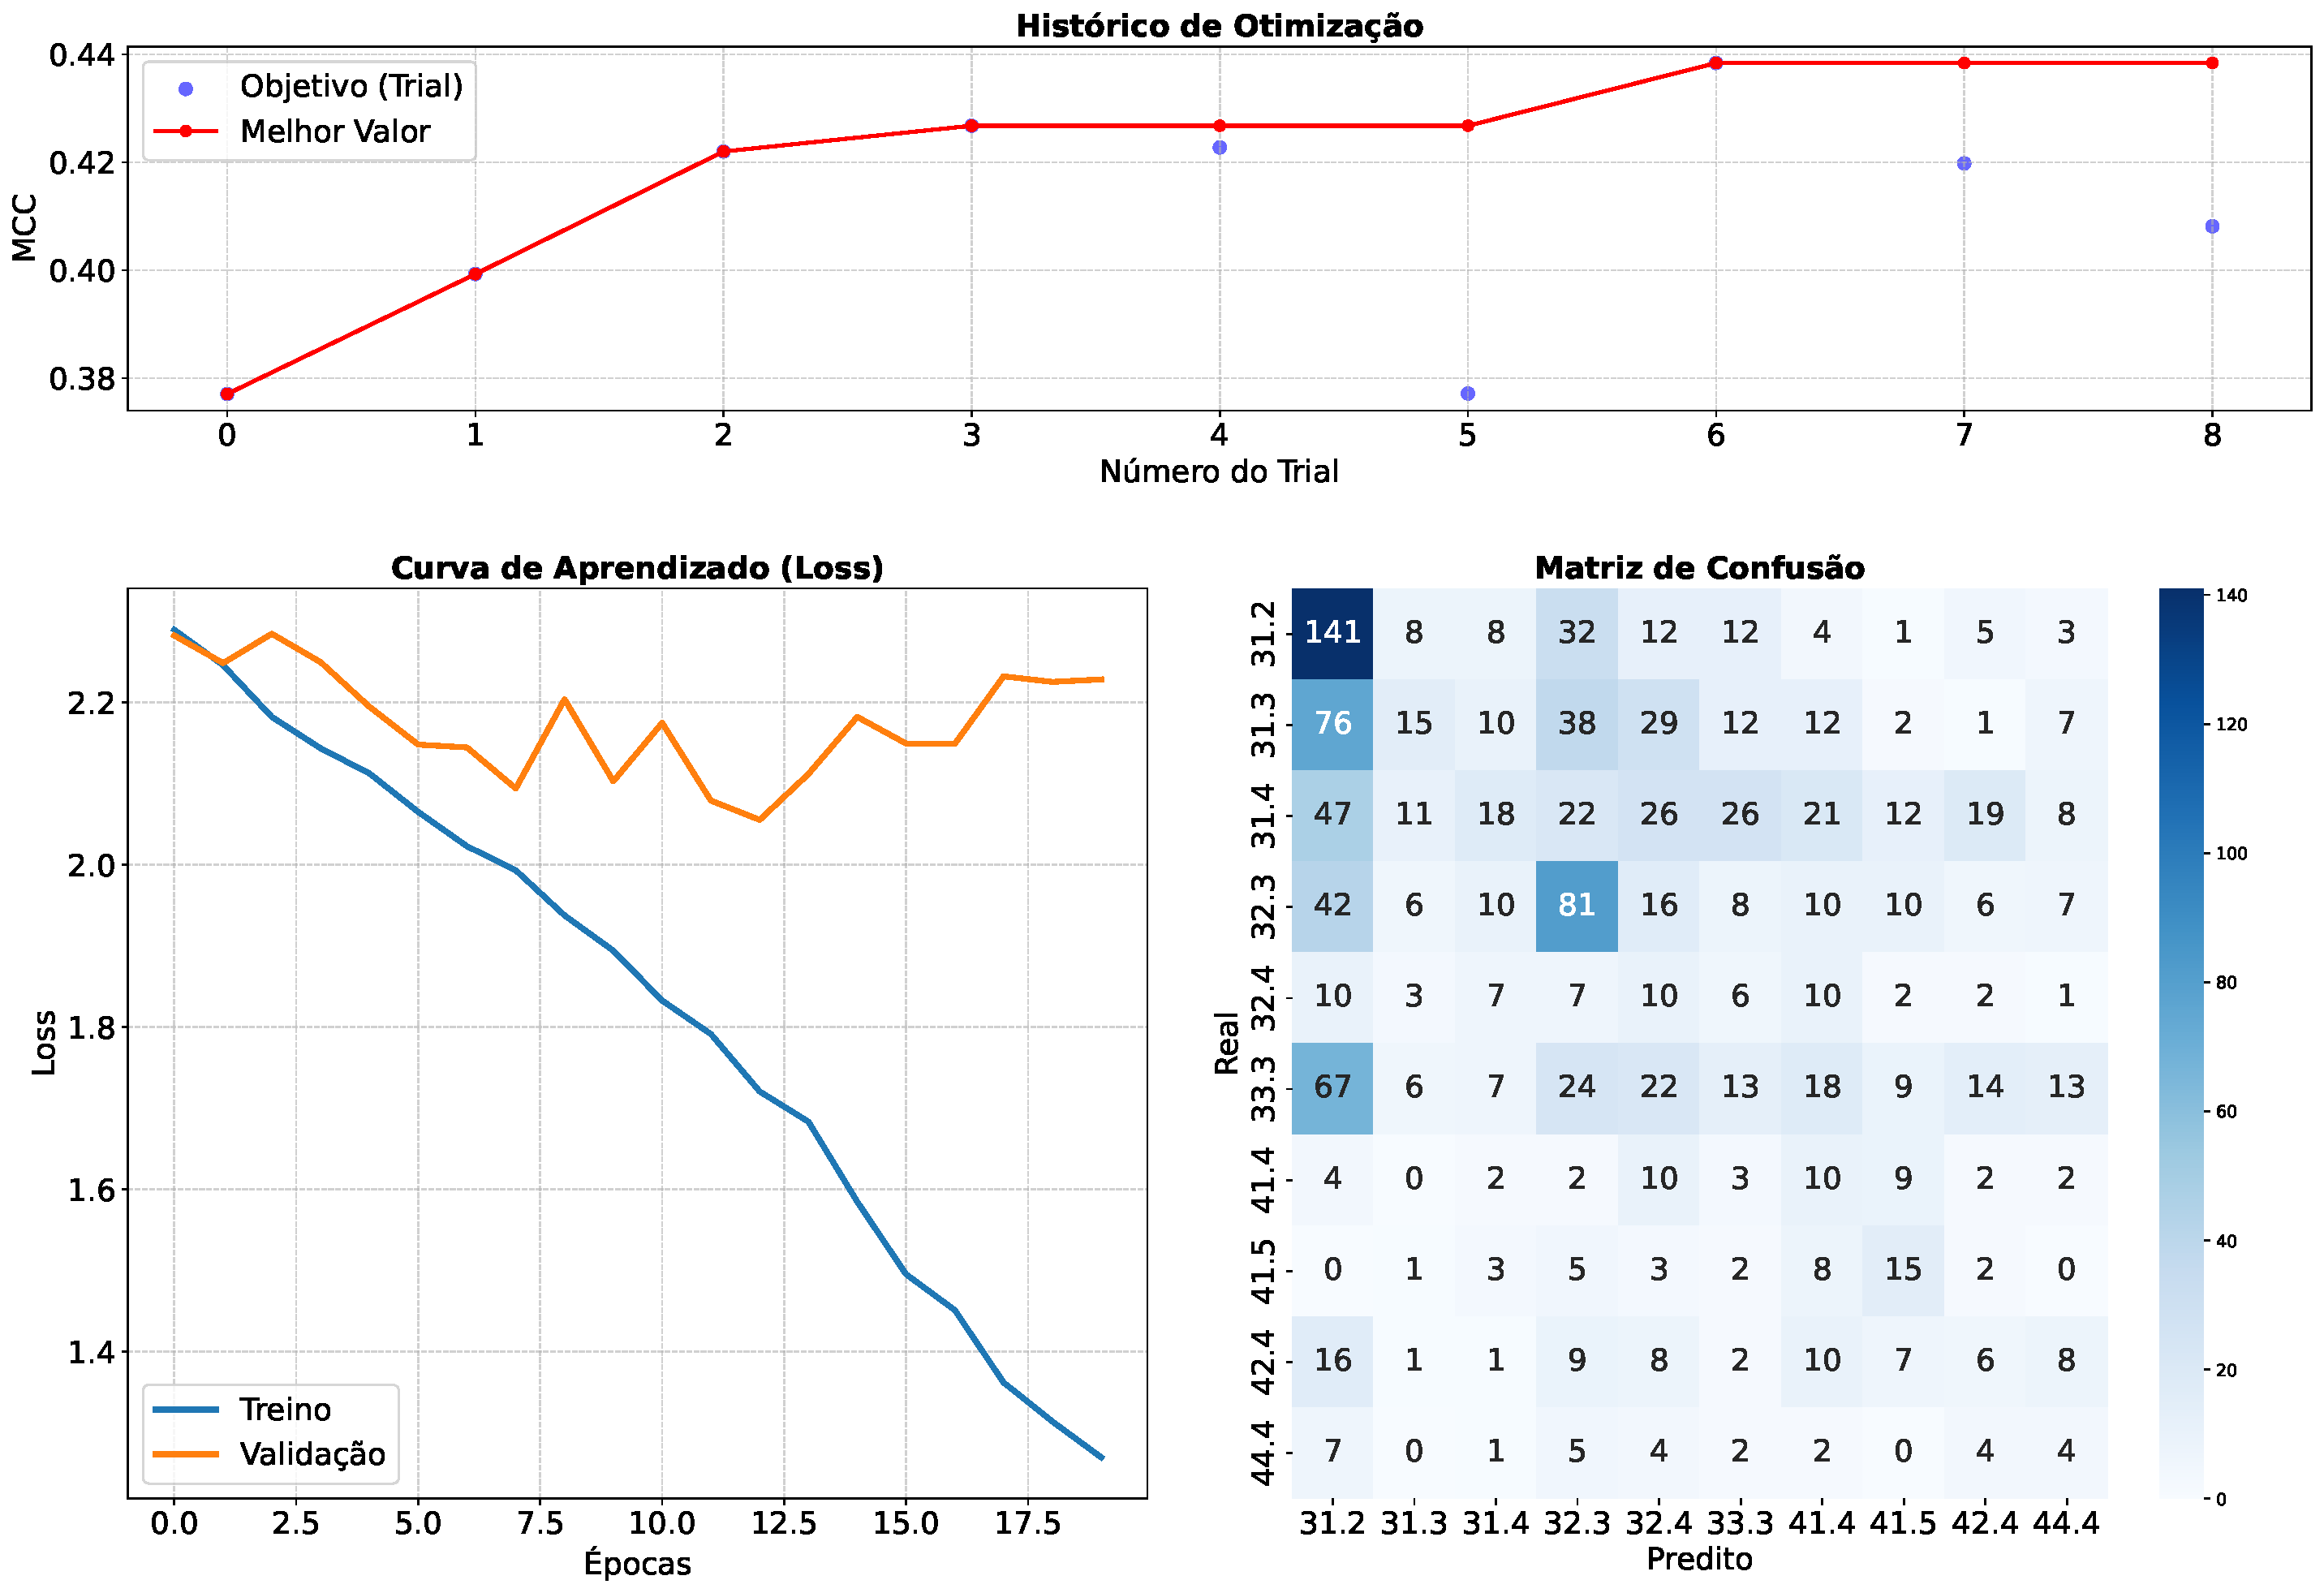
\includegraphics[width=0.85\textwidth]{tex/appendix/experiments/vit_v11_AM_opt_aug/dashboard_consolidado.pdf}
        \caption{Histórico de Otimização, Curvas de Aprendizado e Matriz de Confusão - vit\_v11\_AM\_opt\_aug}
    \end{figure}
\end{minipage}
\clearpage
